\chapter{\color{Millum}\textbf{Innledning}}
\newthought {Som avslutning for bachelorprogrammet ved institutt for teknologi ved Høyskolen Kristiania} har vi gjennomført BAO300 Bachelorprosjekt hos Millum AS. Hensikten med prosjektet er å få erfaring og bruke kunnskap og ferdigheter vi har tilegnet oss gjennom studiene til å gjennomføre en reel oppgave. Vi skal benytte relevant forskning og demonstrere bruk av teknologi, verktøy og metode for utvikling og prosjektstyring.

Prosjektet omhandler planlegging, utvikling og lansering av en mobilapplikasjon knyttet varetellingsmodulen i handelsportalen "Millum Procurement".

\section{\textbf{Om gruppen}}
Vår bachelorgruppe består av tre studenter ved Institutt for teknologi ved Høyskolen Kristiania. Vi har alle en teknisk sterk bakgrunn og alderen strekker seg mellom 22 og 27 år. Andreas og Erik studerer intelligente systemer, og Vetle studerer frontend- og mobilutvikling. Vi har med bakgrunn i studieretningene våre bred kompetanse innenfor systemutvikling og prosjektstyring.

\begin{table}[htbp]
  \centering
  \caption{Oversikt over gruppemedlemmer}
    \begin{tabular}{|l|l|p{17.355em}|}
    \toprule
    Navn & Rolle & Arbeidsoppgaver \\
    \midrule
    \multicolumn{1}{|p{6.43em}|}{Andreas Eilertsen \newline{}Lybo} & \multicolumn{1}{p{7.215em}|}{Scrum master og\newline{}integrasjonsarkitekt} & Ansvarlig for å koordinere prosjektet opp mot arbeidsgiver, sørge for fremdrift i prosjektet og være ansvarlig for integrasjonen\newline{} mot Millum sine systemer. \\
    \midrule
    Erik Valderhaug & Utvikler & Ansvarlig for utvikling og \newline{}implementasjon av design. \\
    \midrule
    Vetle Stubberud & UX- og fagansvarlig & Ansvarlig for utarbeiding av skisser, \newline{}brukeropplevelse og flyt i applikasjonen, og \newline{}fagansvarlig. \\
    \bottomrule
    \end{tabular}%
  \label{tab:addlabel}%
\end{table}%

\section{\textbf{Beskrivelse av prosjektet}}

\newthought {I dag gjennomfører mange bedrifter varetellinger med penn og papir, eller med dyre håndterminaler.} Hensikten med å gjennomføre en varetelling er å kartlegge summen av varelageret slik at det kan føres inn i regnskapet til bedriften. Det er nemlig slik at balanseregnskapet viser et slags ''øyeblikksbilde'', og for varetellingen vil det resultere i en oversikt over virksomhetens omløpsmidler . Ettersom alt blir regnskapsført vil dette også direkte påvirke bedriftens reelle verdi. I tillegg er det å gjennomføre en varetelling også verdifullt for de som sitter på innkjøpssiden. Om det gjelder matvarer med lang utløpsdato, vil det igjen være bra for å hindre for eksempel matsvinn.

Det å planlegge og gjennomføre varetellinger er ofte lange og dyre prosesser for bedriftene og Millum har utviklet en ny modul i sin handelsløsning Millum Procurement for å gjennomføre varetellinger koblet opp mot deres systemer. De ønsker videre å utvikle en mobilapplikasjon for denne nye modulen, og vårt prosjektet omhandler hele prosessen fra forarbeid og research, til utvikling og publisering av denne mobilapplikasjonen til ulike plattformer.

Siden løsningen rettes mot eksisterende kunder av Millum, som bruker deres handelsløsninger daglig ønsker arbeidsgiver at vi gjennomfører spørreundersøkelser blant deres kunder for å kartlegge hva slags enheter og operativsystem de bruker slik at vi utvikler målrettet mot disse. Videre ønsker de at produktet designes og utvikles på en slik måte at den passer inn i produktporteføljen deres.


\section{\textbf{Introduksjon av oppdragsgiver}}
\newthought {Millum AS er et markedsledende norsk teknologiselskap som leverer e-handelsløsninger til storhusholdningsbransjen.} Selskapet ble etablert i 2002 og har i underkant av 30 ansatte fordelt på avdeling for utvikling, kundeservice, marked- og business. Målene til Millum er å levere fremragende kundeopplevelser som skaper bærekraftige konkurransefortrinn for sine kunder. Selskapet opererer per 2020 i Norge, Sverige og Danmark. For mer informasjon besøk \textbf{\url{https://www.millum.no}}.

\begin{table}[htbp]
  \centering
  \caption{Oversikt over personer involvert i prosjektet utenom gruppemedlemmer}
    \begin{tabular}{|l|l|p{17.355em}|}
    \toprule
    Navn & Rolle & Tilknytning \\
    \midrule
    \multicolumn{1}{|p{6.43em}|}{Hans Kristian \newline{}Rygh} & \multicolumn{1}{p{7.215em}|}{Systemarkitekt og\newline{}veileder} & Millum AS \\
    \midrule
    Fredrik L. Brauti & Prosjektleder & Millum AS \\
    \midrule
    Boye J. Kolstad & Produkteier & Millum AS \\
    \midrule
    Sandra K. Murzynowska & UX / QA-ansvarlig & Millum AS \\
    \midrule
    Sturla Bakke & Veileder & Høyskolen Kristiania \\
    \bottomrule
    \end{tabular}%
  \label{tab:addlabel}%
\end{table}%

\section{\textbf{Oppdragsgivers ønsker}}
\newthought{I samarbeid med oppdragsgiver og scrum master i bachelorgruppen} ble det tidlig i prosessen utarbeidet et sett med ønsker om funksjonalitet utformet som user stories. Det er ut ifra disse at oppdragsgiver vurderer leveransene vår underveis og ved en endelig leveransetest av prosjektet. Listen strekker seg fra innlogging via deres systemer, til håndtering av ulike scenarioer i mobilapplikasjonen. Oppdragsgiver har gitt oss ganske frie tøyler til å løse disse oppgavene, men vi involverer likevel nøkkelpersoner fra bedriften underveis i hele prosjektet.

\begin{figure}[H] 
    \centering
    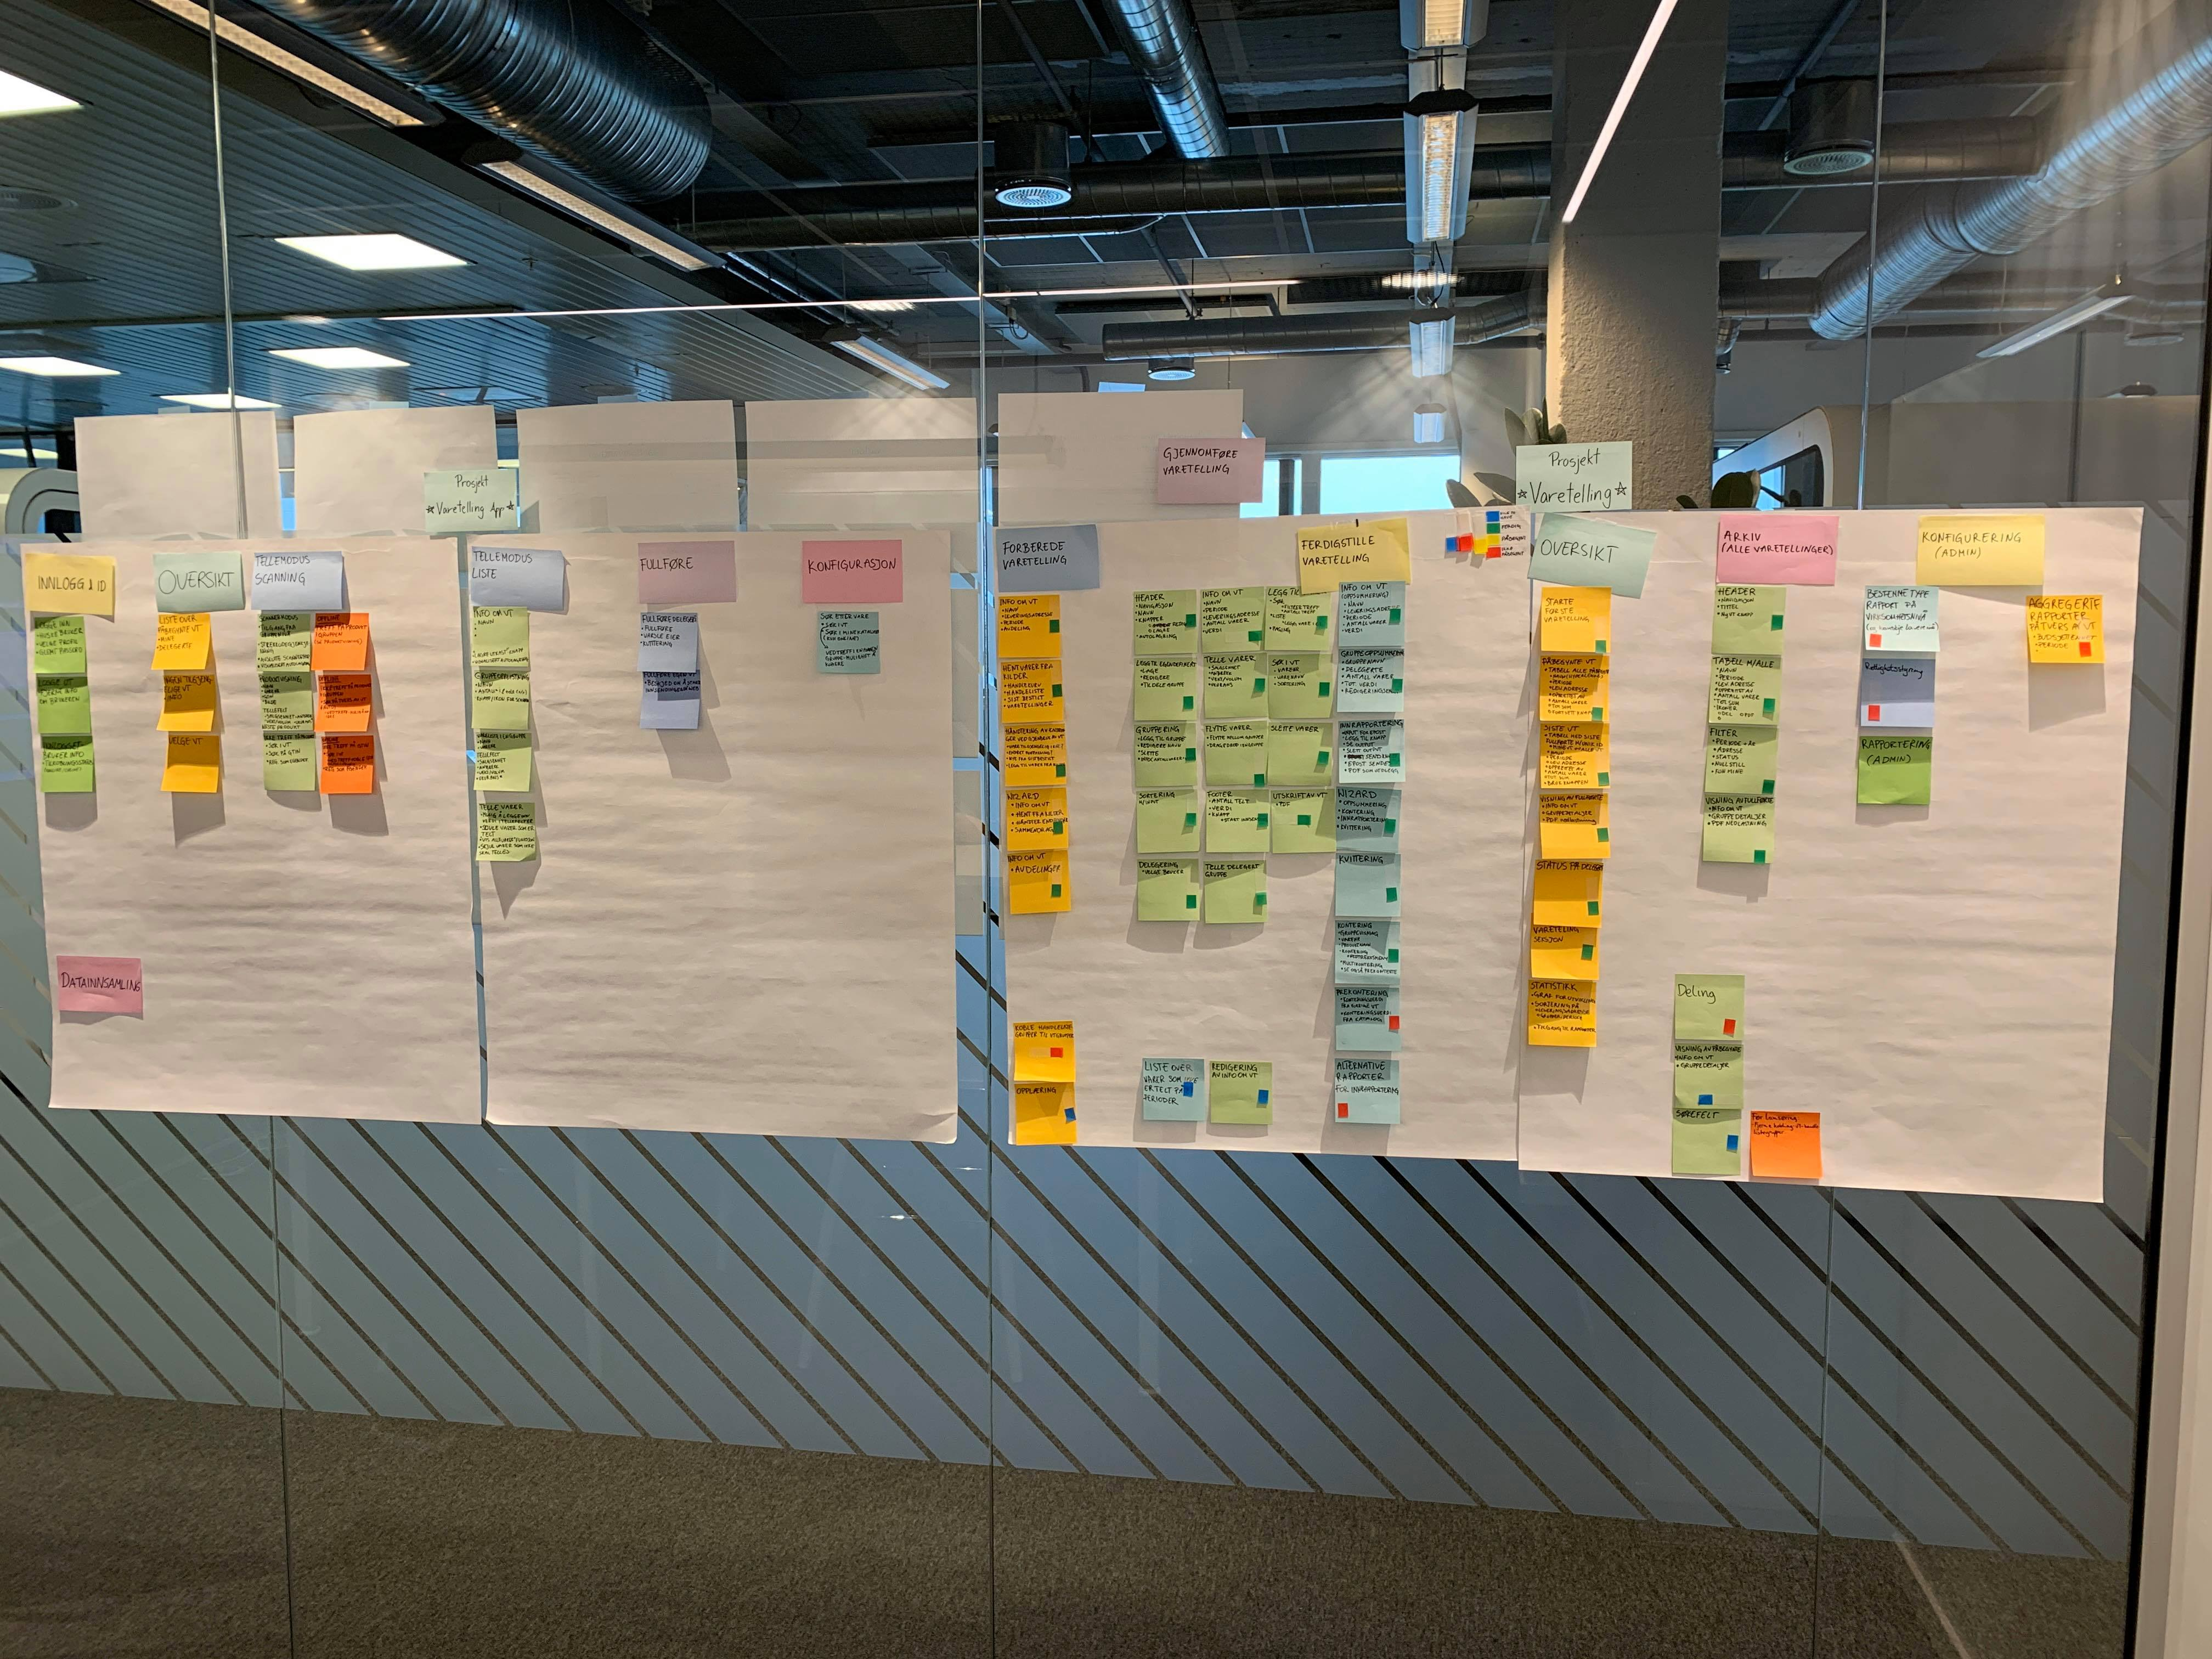
\includegraphics[width=\textwidth]{figures/Innledning/post-it.jpg}
    \caption{User stories knyttet til prosjektet}
\end{figure}

\section{\textbf{Ambisjoner}} \label{Ambisjoner}
I forbindelse med oppstarten av prosjektet satte gruppen seg ambisjonsmål, både akademisk og til å løse oppdragsgivers ønsker. Listen under er sortert fra viktigste til minst viktige ambisjon.

\begin{description}
    \item[$\cdot$ Utvikle en løsning som reduserer tid og kostnad ved gjennomføring av varetellinger.] og løser problematikken mange av Millums kunder opplever i dag.
    \item[$\cdot$ Levere en god akademisk oppgave]som står til de forventningene Høyskolen har til sine bachelorstudenter. Vi har også satt oss et ambisjonsmål om å levere godt nok til å få en B eller bedre.
    \item[$\cdot$ Få erfaring]med hele prosessen i et prosjekt fra innsikt og analyse til leveranse og handover.
    \item[$\cdot$ Personlig utvikling.]Både profesjonelt ved å skape et større nettverk, og personlig ved å få mestringsfølelse.
\end{description}

\section{\textbf{Teoretisk forankring}} \label{TeoretiskForankring}

Gjennom prosjektet har vi støttet oss på flere litteratur- og nettkilder til flere emner. I dette kapittelet vil introdusere vår teoretiske forankring. 

\subsection{\textbf{Prosess og metode}}
Litteratur vi har benyttet i forbindelse med prosess og metode.

\begin{description}
    \item \textbf{Essential Scrum: A Practical Guide to the Most Popular Agile Process}
     
     Dette er en bok vi tidligere har brukt da vi lærte om Scrum og har blitt benyttet seg som et oppslagsverktøy.
    
    \item \textbf{Researching Information Systems and Computing}
    
     Oates har skrevet denne boken i forbindelse med hvordan man kan utføre et forskningsprosjekt og har blitt benyttet av oss i forbindelse med gjennomføring av støtteemnet ``Undersøkelsesmetoder``.

\end{description}


\subsection{\textbf{Design og utforming}}
Litteratur knyttet til design og utforming:

\begin{description}

    \item \textbf{Univeral Principles of Design}
    Boken tar for seg en rekke viktige designprinsipper og har blitt valgt ettersom den etterhvert har begynt å bli sett på som en standard innenfor design. Den inneholder en rekke viktige designprinsipper som vi har fulgt gjennom utviklingsprosjektet.

    \item \textbf{Don't Make Me Think: A Common Sense Approach to Web Usability}
    En av de første og beste bøkene skrevet om design prinsippet \textit{usability}. Boken er vår hovedreferanse til emnet Usability. 
    
    \item \textbf{Nielsen Norman Group}
    NNG er verdensledene i forskningsbasert brukeropplevelse, og har vært et supplement til bøkene \textit{Don't Make Me Think} og \textit{Universal Principles of Design}.
  

\end{description}





\subsection{\textbf{Tekniske valg}}
Litteratur og kilder til teknisk teori:

\begin{description}
    \item \textbf{Design patterns: elements of reusable object-oriented software}
    
    \item \textbf{Ionic og Angular sin dokumentasjon}
    
    Vi har i tillegg tatt i bruk de offisielle dokumentasjonene til teknologiene vi har brukt. 

\end{description}


